\section{Fundamentos de estructuras metal óxido semiconductor}
La estructura MOS es la base de la tecnología de 
circuitos integrados modernos\cita{sze_physics_2007}
que componen las PCs, dispositivos móviles e infraestructura de comunicaciones.
Su forma de fabricación, denominada proceso CMOS,
ha permitido un crecimiento exponencial en la capacidad de cómputo,
gracias a la constante miniaturización de los transistores que componen un
circuito integrado (\figref{fig:moore}).
\fig{moore}{figuras/moore/moore.pdf}
{Reducción exponencial de las dimensiones del transistor.
La cantidad de transistores en un microprocesador se duplica cada dos años 
siguiendo la ley de Moore\cite{moore_cramming_2006}.
Reproducido de \cite{sedra_microelectronic_2010}.}
\subsection{Capacitor MOS}
Para entender el transistor MOS, estudiamos antes el capacitor MOS.
Consiste en un sustrato semiconductor donde se deposita un aislante delgado 
(tradicionalmente SiO$_2$ sobre Si)
y un conductor (\emph{gate}) como en la \figref{fig:cortemos}.
Esto forma un capacitor porque tiene dos conductores separados por un
dieléctrico.
\fig{cortemos}{figuras/mos/corte.png}{Corte lateral de una estructura MOS. 
Reproducido de~\cite{sze_physics_2007}.}
%
\subsubsection{Estructura de bandas}
La \figref{fig:bandasmos} muestra la estructura de bandas del MOS ideal.
Un MOS ideal no tiene carga atrapada en el óxido o en la interfaz
óxido-semiconductor, y sus bandas no tienen curvatura cuando no se le aplica
tensión.
Observamos la variación de las bandas en la dirección normal al sustrato,
y su dependencia con la tensión $V$ aplicada.
Al conectar una fuente de tensión (por ejemplo una batería)
entre las terminales, fijamos la diferencia entre el nivel de Fermi del metal y
el del semiconductor. 
El gradiente de $E_F$ produce un desplazamiento de cargas hasta que se llega a
un nuevo equilibrio (\figref{fig:polarizacionmos}).

%Bajo la condición $V=0$, los niveles de Fermi de metal y
%semiconductor coinciden.
%Para cada material, el nivel de vacío $\phi$ 
%está a una distancia fija del nivel de Fermi.
%En un metal esta distancia se denomina función trabajo.
%En un semiconductor esta cantidad es la suma de la afinidad electrónica $\xi$
%(distancia entre la banda de conducción y el nivel de vacío)
%y 
%Por ejemplo, la función trabajo del aluminio es \SI{4.2}{\volt} y la de una
%oblea dopada tipo P típica es \SI{3.6}{\volt}.
%Cuando coinciden los niveles de Fermi de metal y semiconductor, 
%difiere su potencial eléctrico en \SI{0.6}{\volt}.
%$\phi$ varía de forma contínua entre las terminales,
%curvando las bandas.
%Hace falta aplicar una tensión $V_{fb}=(\phi_m-\phi_s)/e$ 
%para obtener bandas planas (que implican, por Poisson, carga nula).
%
\fig{bandasmos}{figuras/mos/bandas.png}
{Estructura de bandas del capacitor MOS en flatband o bandas planas.
Reproducido de~\cite{sze_physics_2007}.}
\begin{figure}[H]
    \centering
    \begin{subfigure}[b]{.3\textwidth}
        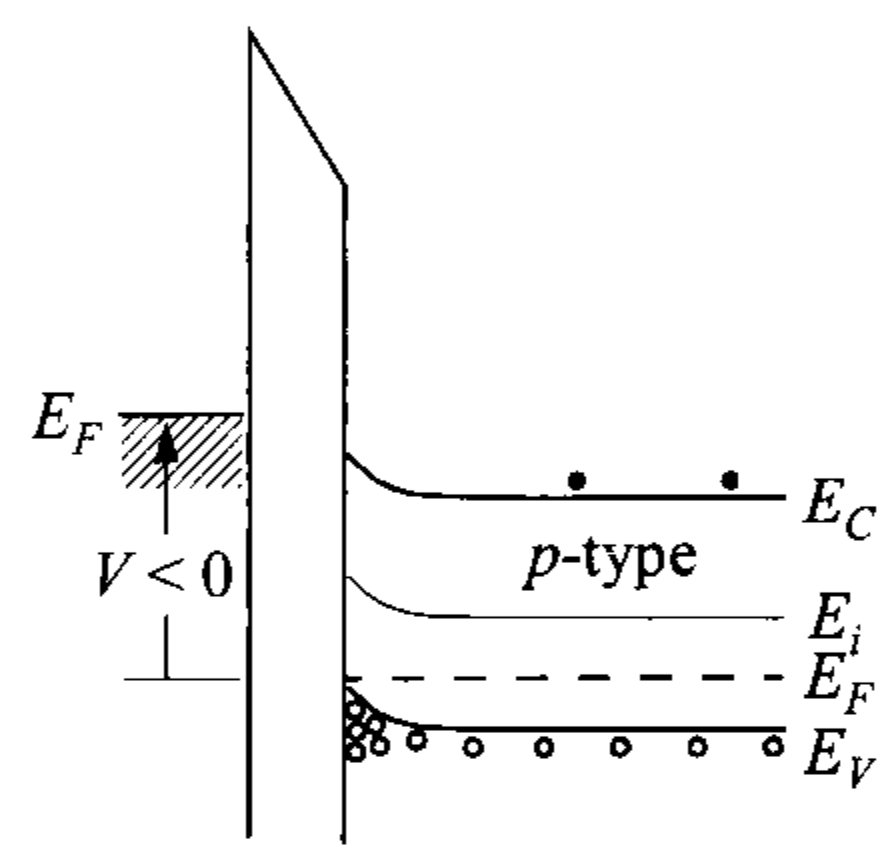
\includegraphics{figuras/mos/acumulacion.png}
        \label{fig:mosacumulacion}
        \caption{Acumulación}
    \end{subfigure}
    \begin{subfigure}[b]{.3\textwidth}
        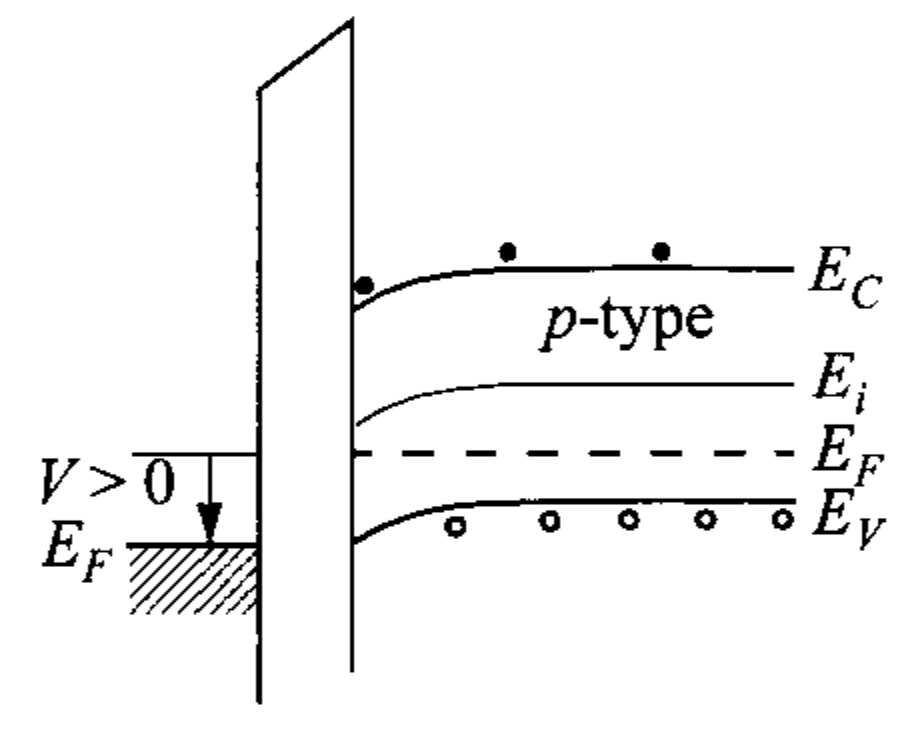
\includegraphics{figuras/mos/desercion.png}
        \label{fig:mosdesercion}
        \caption{Deserción}
    \end{subfigure}
    \begin{subfigure}[b]{.3\textwidth}
        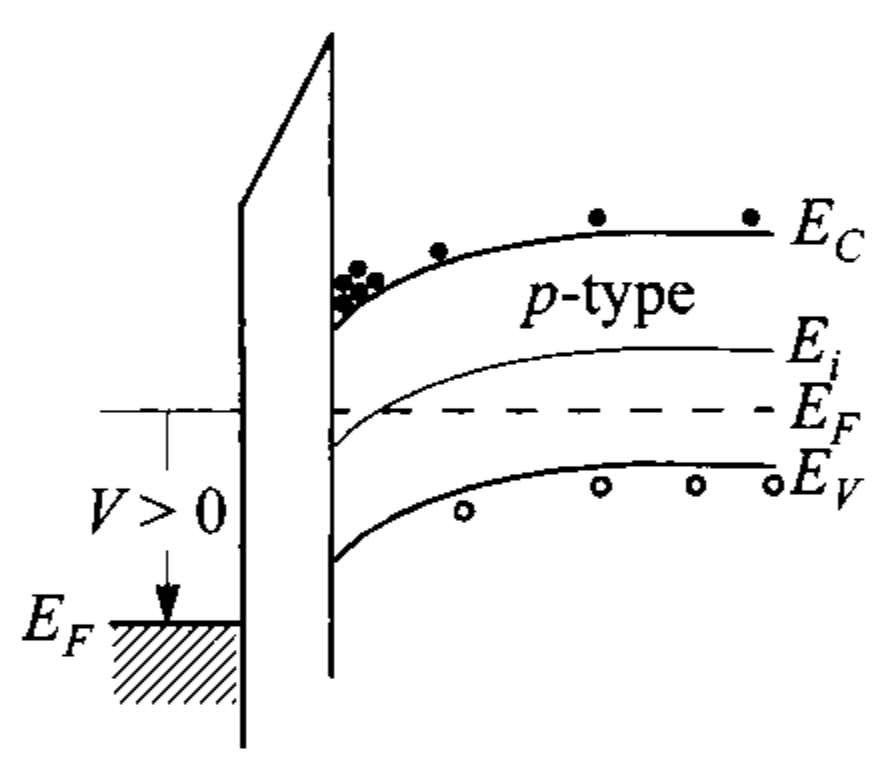
\includegraphics{figuras/mos/inversion.png}
        \caption{Inversión}
        \label{fig:mosinversion}
    \end{subfigure}
    \caption{Bandas del MOS polarizado, para $V_{fb}=0$.
Reproducido de~\cite{sze_physics_2007}.}
    \label{fig:polarizacionmos}
\end{figure}
%
\subsubsection{Relación carga-tensión}
Planteando la ecuación de Poisson para el potencial $\phi$ en el semiconductor se llega a
\begin{align*}
    \deriv{^2\phi}{x^2} &= \frac e{\epsilon_s}(N_d-N_a+p-n),
\end{align*}
siendo los términos de la derecha concentraciones de donantes, aceptores,
huecos y electrones.

Para modelar la concentración de huecos y electrones en semiconductores,
se usa con gran éxito la aproximación de electrón independiente.
La misma permite pensar en términos de niveles de 1 electrón que son ocupados
por electrones idénticos que no interactúan.
La termodinámica de un sistema de electrones
lleva a la estadística de Fermi-Dirac, 
que dice que la ocupación de un nivel está dada por
\begin{align*}
    f(E) = \left[\exp\left(\frac{E-E_F}{kT}\right)+1\right]^{-1}
\end{align*}
con $E$ la energía del nivel y $E_F$ el nivel de Fermi.
$E_F$ es constante a lo largo de un sistema en equilibrio
químico,
y puede despejarse como función del número total de partículas.

En muchos casos se cumple $|E-E_F| \gg kT$,
permitiendo aproximar
\begin{align*}
    f(E) = \exp\left(-\frac{E-E_F}{kT}\right)
\end{align*}.
Es conveniente expresar la dependencia de la concentración d portadores 
con el potencial medido respecto al contacto de bulk
(un punto alejado del semiconductor que tomamos como referencia):
$\psi_p=\phi(x)-\phi(\infty)$,
\begin{align}
    n &= n_0\exp\left(\frac{q\psi_p}{kT}\right)&
    p &= p_0\exp\left(-\frac{q\psi_p}{kT}\right),
    \label{eq:portadores_nodegenerados}
\end{align}
con $n_0$ y $p_0$ las concentraciones de portadores en el bulk.
Estas concentraciones dependen principalmente de la concentración $N_a$ de
impurezas aceptoras de electrones agregadas durante la fabricación.
Típicamente $p_0\approx N_a$ y $n_0\approx n_i^2/N_a$ con $n_i$ la
pequeña concentración intrínsica de portadores.
Esto equivale a decir que todas las impurezas están ionizadas y aportan portadores.
Se debe a que los niveles de impureza se sitúan a varios $kT$ de distancia de
$E_F$.
Por lo tanto, se encuentran casi completamente ionizados 
y muy pocos portadores quedan ligados al ión aceptor.
% FIXME Ashcroft lo explica con Ei << kT

La aproximación~\ref{eq:portadores_nodegenerados} es válida para 
$|E_F-E_{c/v}|\gg kT$, 
o sea el nivel de Fermi alejado de los bordes de las bandas.
Así se obtiene un sistema de ecuaciones cuya solución para el campo eléctrico es
\begin{align*}
    \mathscr{E}_s &= \pm \frac{\sqrt 2kT}{qL_D}
    F(q\psi_p/kT,n_{p0}/p_{p0})\textnormal{, con}\\
    L_D^2&=\frac{kT\epsilon_s}{p_{p0}q^2}\textnormal{ , y}\\
    F(x,y) &= \sqrt{e^{-x}+x-1+y(e^x-x-1)}.
\end{align*}
Usando la ley de Gauss se obtiene la carga total del semiconductor
\begin{align*}
    Q_s = -\epsilon_s\mathscr{E}_s.
\end{align*}
La relación entre $V_G$ y $\psi_p$ viene de plantear la continuidad del vector
desplazamiento y la caída de tensión en el aislante
\begin{align*}
    V_G &= \psi_s + \mathscr{E}\frac{\epsilon_s}{\epsilon_{ox}}t_{ox}.
\end{align*}
Esto resulta en el gráfico de la \figref{fig:cargamos},
donde delimitamos distintos regímenes de operación.
%
\subsubsection{Regímenes de operación del capacitor MOS}
\begin{itemize}
    \item Acumulación:
        Aplicando tensión negativa al gate
        se puebla la superficie de portadores mayoritarios.
    \item Flatband/bandas planas: 
        A \SI{0}{\volt} la carga positiva de los huecos 
        (portadores mayoritarios)
        cancela la carga negativa de los aceptores, 
        entonces $Q=0$. 
    \item Deserción/Inversión débil:
        Aumentando la tensión se vacía la superficie de portadores
        mayoritarios,
        dejando la carga neta negativa de los aceptores ionizados.
    \item Inversión fuerte:
        Al cruzar $2\psi_B$ se puebla la superficie de portadores minoritarios
        con carga negativa,
        de igual magnitud y signo opuesto a la del sustrato.
        Un pequeño aumento adicional de $V_G$ resulta en un aumento exponencial
        de $|Q|$.
        Esta dependencia exponencial es válida hasta que el nivel de Fermi 
        se aproxima al borde de la banda de conducción y 
        el semiconductor se torna degenerado.
        Esto significa que se comporta como un metal,
        con una densidad de portadores que varía levemente con el potencial.
\end{itemize}
\fig{cargamos}{figuras/mos/carga_vg.pdf}{Carga de un MOS típico 
    ($N_A=$\SI{4e15}{\centi\meter^{-3}}) en función
de la tensión de gate.
En la región de la izquierda el nivel de Fermi se acerca a la banda de
valencia. Esto torna degenerado al semiconductor y requiere el uso de
estadística de Fermi-Dirac en vez de aproximarla por Maxwell-Boltzmann.}
%
%
\subsection{Transistor MOS}
El transistor es la base de la electrónica moderna.
Modulando una señal con otra, permite realizar tareas analógicas como
amplificación y multiplicación.
Al operarlo con niveles discretos (prendido/apagado),
permite realizar las operaciones lógicas básicas (NOT, AND, etc.) que
se combinan para formar un circuito digital.
Su evolución permitió la integración de un número creciente de funciones
digitales y analógicas en un mismo circuito integrado.
%
\subsubsection{Modelo circuital}
El MOSFET o transistor MOS es un dispositivo con 4 terminales:
drain, gate, source y body (\figref{fig:mosfetschem}).
\fig{mosfetschem}{figuras/mos/mosfet.pdf}{Símbolo esquemático del transistor MOS.}
Frecuentemente se conecta source con body, rompiendo la simetría source-drain.
La tensión entre gate y source controla la corriente drain-source.

En la \figref{fig:mosfetoutput} se ven los 3 modos de operación del MOS:
\fig{mosfetoutput}{figuras/mos/output.pdf}{Curvas características de un
transistor MOS típico.}
\begin{itemize}
    \item Corte: Si $V_g<V_T$, no fluye corriente de drain.
        Por eso esta es denominada la ``tensión umbral''.
        $V_T$ es un parámetro de fabricación que ronda \SI{.3}{\volt} en procesos CMOS
        modernos.
    \item Triodo: Si $V_g>V_T$ y $V_{ds}<V_g-V_T$, la corriente de drain crece con la
        tensión drain-source siguiendo
        \begin{align*}
            I_D&=\beta_n\frac WL(V_{gs}-V_T-\frac{V_{ds}}2)V_{ds},
        \end{align*}
        con $\beta_n$ un parámetro del proceso y $\frac WL$ la relación de
        aspecto del MOSFET.
    \item Saturación: Si $V_g>V_T$ y $V_{ds}>V_g-V_T$ la corriente se mantiene, a primer
        orden, al valor constante
        \begin{align*}
            I_{Dsat}&=\frac{\beta_n}2\frac WL(V_{gs}-V_T)^2.
        \end{align*}
\end{itemize}
%
\subsubsection{Modelado físico}
El MOSFET de canal n consiste en un capacitor MOS de sustrato p entre dos regiones fuertemente dopadas 
tipo n, 
que forman drain y source (\figref{fig:mosfetestructura}).
Sin tensión de gate no puede fluir corriente entre drain y source porque una de las
junturas p-n (drain-sustrato o source-sustrato) queda polarizada en inversa.

Al polarizar el MOS en inversión se forma junto al óxido
de gate una capa de electrones libres llamada canal.
Esta región de tipo n conecta drain y source y permite el flujo de corriente.
Al variar la tensión de gate, la variación de carga en el canal modula su
conductividad.
% TODO: deducir ecuaciones?
\fig{mosfetestructura}{figuras/mos/mosfet.png}{Estructura del transistor MOS.
Reproducido de~\cite{sze_physics_2007}.}
